\newpage
\definecolor{lblue}{rgb}{0.39, 0.58, 0.93}
%\blfootnote{\color{toancuabi}$^1$Đại học Thăng Long.}
\everymath{\color{toancuabi}}
\graphicspath{{../timhieucungbi/demtamgiac1/}}
%\begingroup
%\AddToShipoutPicture*{\put(125,520){
\includegraphics[scale=0.75]{tieude1.pdf}}} 
%\centering
%\endgroup
%\vspace*{15pt}
	\begin{center}
		\textbf{\Large\color{toancuabi}NHỮNG BÀI TOÁN ĐẾM TAM GIÁC}
		
		\vspace*{5pt}
		NGUYỄN THỊ NHUNG
	\end{center}

	Nhiều bạn nhỏ chúng ta khi tham gia các cuộc thi Toán hẳn đã không ít lần gặp khó khăn với những bài toán đếm hình. Khi số lượng hình lớn, đôi khi ta đếm xong rồi vẫn không chắc là mình đếm đã đủ chưa, có đếm lặp hình nào không? Trong bài viết này, chúng ta sẽ cùng nhau tìm hiểu về một số dạng bài toán đếm tam giác, rút ra những “mẹo” đếm để không rơi vào tình cảnh “đếm vài lần, mỗi lần một kết quả” nhé.
	\vskip 0.1cm
	Trước hết, chúng ta giới thiệu một vài tên gọi sẽ dùng chung trong các phần dưới đây.
	\vskip 0.1cm
	-- \textbf{\color{toancuabi}Tam giác đơn}: tam giác không chứa tam giác nào bên trong;
	\vskip 0.1cm
	-- \textbf{\color{toancuabi}Tam giác đôi}: tam giác tạo ra từ $2$ tam giác đơn;
	\vskip 0.1cm
	-- \textbf{\color{toancuabi}Tam giác ba}: tam giác tạo ra  từ $3$ tam giác đơn;
	\vskip 0.1cm
	-- \ldots
	\vskip 0.1cm
	-- \textbf{\color{toancuabi}Tam giác $\pmb{n}$}: tam giác tạo ra từ $n$ tam giác đơn.
	\vskip 0.1cm
	Bây giờ, chúng ta bắt đầu với một nhiệm vụ đếm tam giác đầu tiên. Nhiệm vụ này khá cơ bản mà chắc bất kỳ bạn nhỏ nào cũng đã từng hoàn thành rồi.
	\vskip 0.1cm
	\textbf{\color{toancuabi}Bài toán $\pmb{1.}$ Đếm số tam giác khi tam giác bị chia thành nhiều phần từ một đỉnh.}
	\vskip 0.1cm
	\textbf{\color{toancuabi}Ví dụ} $\pmb{1.}$ \textit{Hãy đếm số tam giác trong các hình sau.}
	\begin{figure}[H]
		\centering
		\vspace*{-5pt}
		\captionsetup{labelformat= empty, justification=centering}
		\captionsetup[subfigure]{labelformat=empty}
		\hfill\subfloat[\textit{\color{toancuabi}Hình} $1.$]{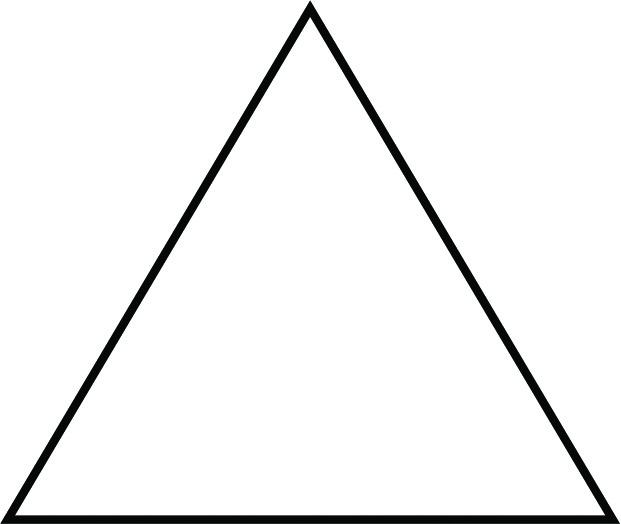
\includegraphics[width=0.2\textwidth]  
			{Tam_giac_1}}
		\hfill
		\subfloat[\textit{\color{toancuabi}Hình} $2.$]{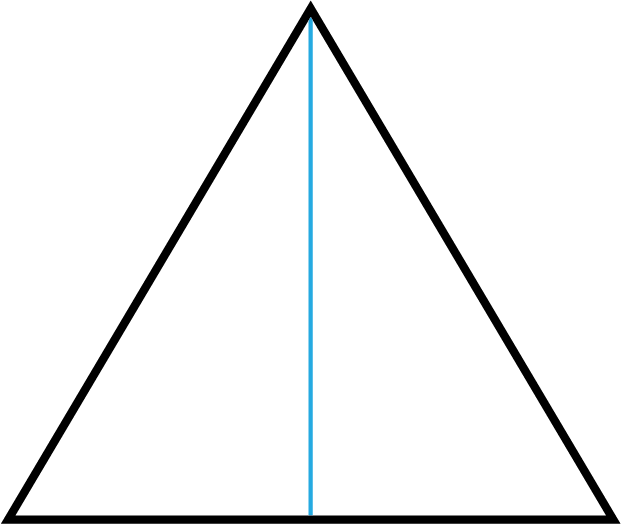
\includegraphics[width=0.2\textwidth]{Tam_giac_2}}
		\hfill
		\subfloat[\textit{\color{toancuabi}Hình} $3.$]{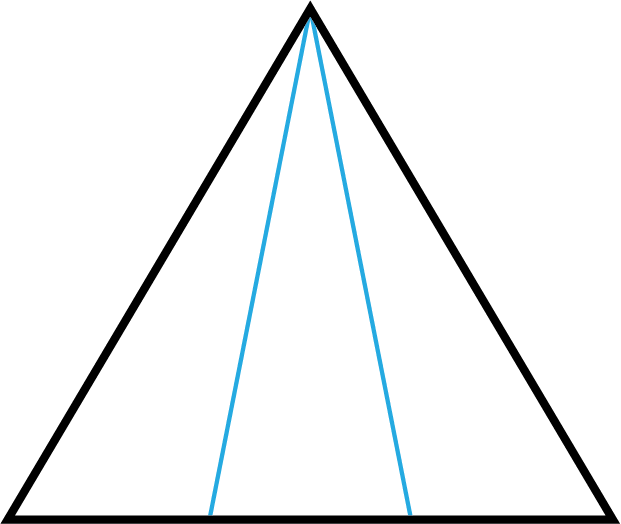
\includegraphics[width=0.2\textwidth]{Tam_giac_3}}\hfill
		\vspace*{-10pt}
	\end{figure}
	\textbf{\color{toancuabi}Lời giải.} Đây là một yêu cầu đếm tam giác khá đơn giản. Phương pháp phổ biến mà các bạn nhỏ thường làm là đánh số các tam giác đơn, sau đó liệt kê từng cách kết hợp hình theo quy tắc từ ít tam giác đơn nhất đến nhiều tam giác đơn nhất. Tiếp đến là đếm số lượng từng loại và cuối cùng cộng các kết quả lại với nhau. Để cho gọn, ta trình bày các bước làm trên theo Bảng $1$.
	\begin{figure}[H]
		\centering
		\vspace*{-5pt}
		\captionsetup{labelformat= empty, justification=centering}
		\captionsetup[subfigure]{labelformat=empty}
		\hfill\subfloat[\textit{\color{toancuabi}Hình} $1$.]{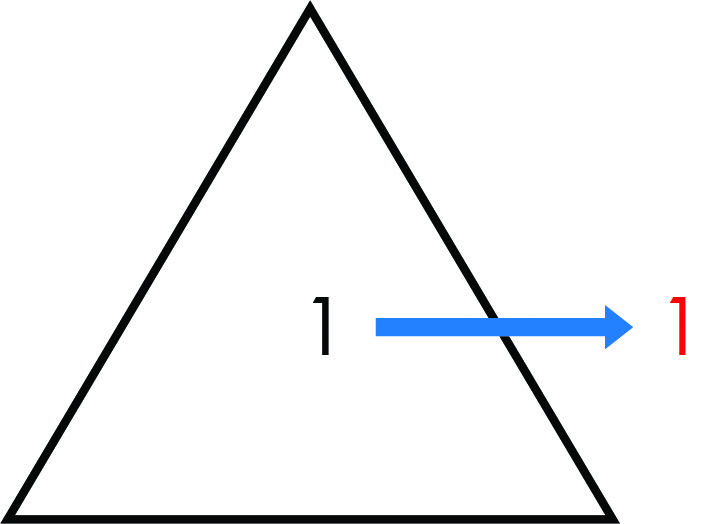
\includegraphics[width=0.2\textwidth]  
			{Tam_giac_1_giai}}
		\hfill
		\subfloat[\textit{\color{toancuabi}Hình} $2$.]{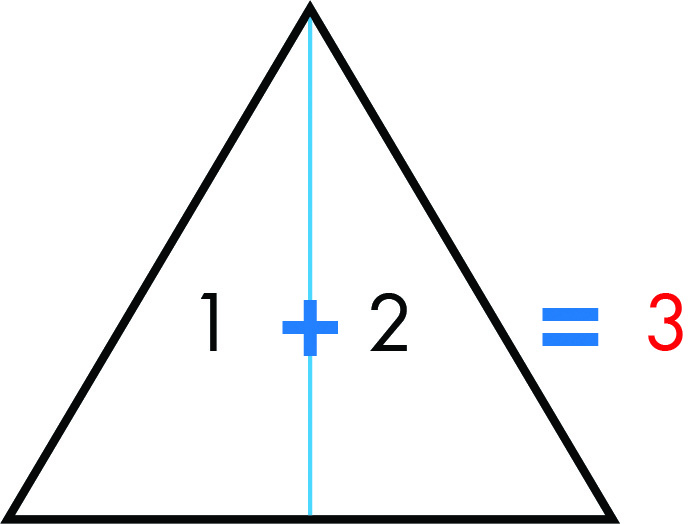
\includegraphics[width=0.2\textwidth]{Tam_giac_2_giai}}
		\hfill
		\subfloat[\textit{\color{toancuabi}Hình} $3$.]{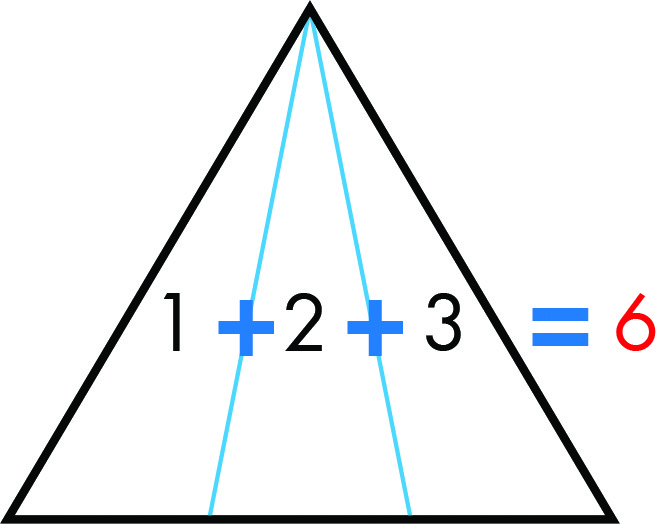
\includegraphics[width=0.2\textwidth]{Tam_giac_3_giai}}\hfill
		\vspace*{-10pt}
	\end{figure}   
	\setlength{\tabcolsep}{5pt}
	\renewcommand{\arraystretch}{1.3}
	\begin{table}[H]
		\vspace*{-5pt}
		\captionsetup{labelformat= empty, justification=centering}
		\resizebox{1\textwidth}{!}{\begin{tabular}{|c|c|c|c|c|c|c|}
				\hline
				\multirow{2}{4em}{\centering{Loại tam giác}}&\multicolumn{2}{c|}{Hình $1$}&\multicolumn{2}{c|}{Hình $2$}&\multicolumn{2}{c|}{Hình $3$}\\
				\cline{2-7}
				&Liệt kê & Số lượng & Liệt kê & Số lượng & Liệt kê & Số lượng\\
				\hline
				Tam giác đơn & $(1)$ & $1$ & $(1)$, $(2)$& $2$ &$(1), (2), (3)$& $3$\\
				\hline
				Tam giác đôi & & &$(1+2)$ &$1$&$(1+2),(2+3)$&$2$\\
				\hline
				Tam giác ba& &&&&$(1+2+3)$&$1$\\
				\hline
				Tổng & &$\color{red}1$&&$\color{red}3 = 2 +1$& &$\color{red}6=3 +2 +1$\\
				\hline
		\end{tabular}}
		\caption{\textit{\color{toancuabi}Bảng $1$.}}
		\vspace*{-10pt}
	\end{table}
	Như ta đã nói ở trên, việc đếm số tam giác trong các hình ở Ví dụ $1$ là khá đơn giản. Tuy nhiên, việc đếm sẽ trở nên khó khăn, mất thời gian và đặc biệt là dễ nhầm lẫn hơn khi tam giác bị chia thành nhiều phần hơn, chẳng hạn thành $4$, $5$ hay nhiều phần hơn nữa. Do đó, chúng ta cần phải tìm ra những “mẹo” đếm hình hay những “câu thần chú”, mà khi gặp một tam giác bất kỳ kiểu này, ta chỉ cần đọc “câu thần chú” này lên là lập tức có kết quả chuẩn luôn. 
	\vskip 0.1cm
	Trong bài viết này, các bạn nhỏ sẽ thấy những “câu thần chú” không phải có ông tiên nào hiện lên cho ta hay “mẹo” đếm hình không phải là từ trên trời rơi xuống, mà là do ta tự tìm ra đấy. Kết quả này xuất phát từ việc ta đếm trên những hình với số lượng nhỏ các tam giác, rồi quan sát, nhận xét và từ đó rút ra quy luật để áp dụng cho những hình phức tạp hơn. Những quy luật này chính là những “câu thần chú” giúp ta đếm hình không những chính xác mà còn rất nhanh nữa. 
	\vskip 0.1cm
	Quay lại Ví dụ $1$, từ bảng liệt kê số kiểu tam giác, ta thấy
	\vskip 0.1cm
	-- Hình $1$: Tam giác bị chia thành $1$ phần: có $1$ tam giác;
	\vskip 0.1cm
	-- Hình $2$: Tam giác bị chia thành $2$ phần: có $1 + 2 = 3$ tam giác;
	\vskip 0.1cm
	-- Hình $3$: Tam giác bị chia thành $3$ phần: có $1 + 2 + 3 = 6$ tam giác.
	\vskip 0.1cm
	Từ đây, chắc các bạn nhỏ đã rút ra được “câu thần chú” rồi đúng không? “Câu thần chú” đầu tiên của chúng ta là:
	\vskip 0.1cm
	\textbf{\color{toancuabi}Quy tắc} $\pmb{1.}$  \textit{Nếu một tam giác bị chia làm $\pmb{n}$ phần từ $1$ đỉnh thì số tam giác là:}
	\begin{align*}
	\color{red} 1+2+\ldots+n = \frac{n(n+1)}{2}.
	\end{align*}
	Thật là đơn giản đúng không các bạn. Chúng ta hãy dùng “câu thần chú” vừa tìm được vừa rồi để làm bài tập sau nhé.
	\vskip 0.1cm
	\textbf{\color{toancuabi}Bài tập} $\pmb{1.}$ \textit{Tìm số tam giác trong Hình $4$ và Hình $5$ dưới đây.}
	\begin{figure}[H]
		\centering
		\vspace*{-5pt}
		\captionsetup{labelformat= empty, justification=centering}
		\captionsetup[subfigure]{labelformat=empty}
		\hfill
		\subfloat[\textit{\color{toancuabi}Hình} $4$.]{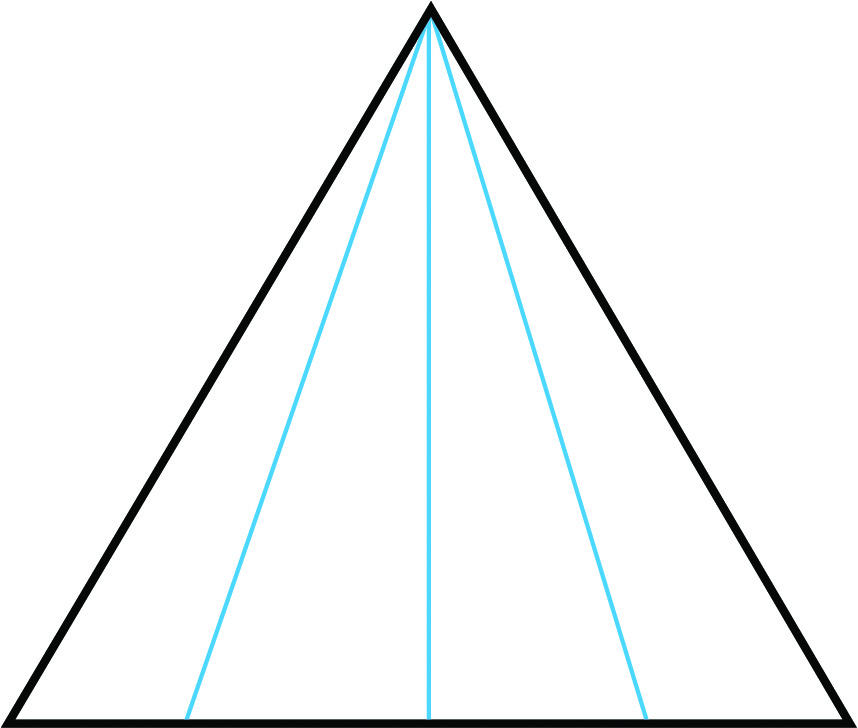
\includegraphics[width=0.2\textwidth]  
			{Tam_giac_4}}
		\hfill
		\subfloat[\textit{\color{toancuabi}Hình} $5$.]{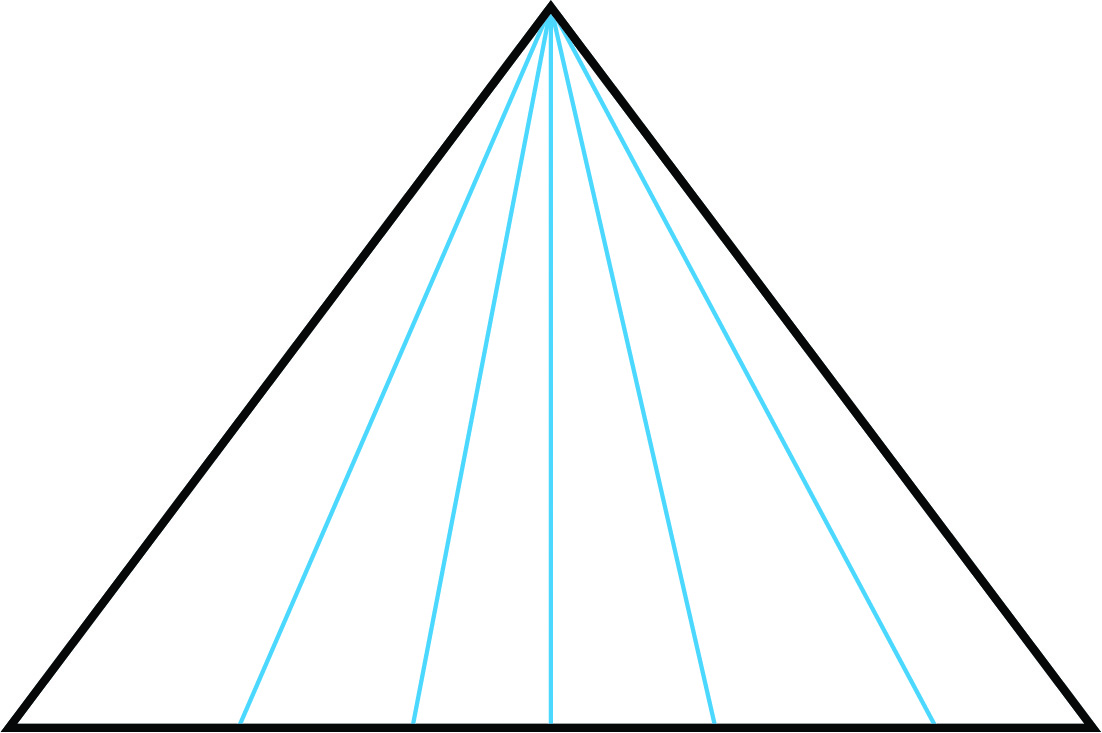
\includegraphics[width=0.28\textwidth]{Tam_giac_5}}
		\hfill
		\vspace*{-10pt}
	\end{figure}   
	Một số bạn nhỏ có thể thắc mắc: Liệu những quy tắc như trên có đúng cho mọi $n$ hay không? Ta mới làm có vài trường hợp của $n$ thôi mà. Nếu bạn nhỏ nào đưa ra thắc mắc này thì rất có “tố chất” của nhà toán học đấy! Các bạn hãy yên tâm dùng những “câu thần chú” trong bài viết này nhé. Sau này khi học lên lớp cao hơn, chúng ta có thể dùng phương pháp quy nạp toán học để chứng minh chặt chẽ những quy tắc như trên.
	\vskip 0.1cm
	Chúng ta cùng tiếp tục với nhiệm vụ thứ hai về đếm tam giác.
	\vskip 0.1cm
	\textbf{\color{toancuabi}Bài toán $\pmb{2.}$ Đếm số tam giác khi tam giác bị chia bởi nhiều phần từ một đỉnh và các đoạn thẳng nằm ngang}
	\vskip 0.1cm
	\textbf{\color{toancuabi}Ví dụ} $\pmb{2.}$ \textit{Hãy đếm số tam giác trong các hình sau}.
	\begin{figure}[H]
		\centering
		\vspace*{5pt}
		\captionsetup{labelformat= empty, justification=centering}
		\captionsetup[subfigure]{labelformat=empty}
		\hfill\subfloat[\textit{\color{toancuabi}Hình} $6$.]{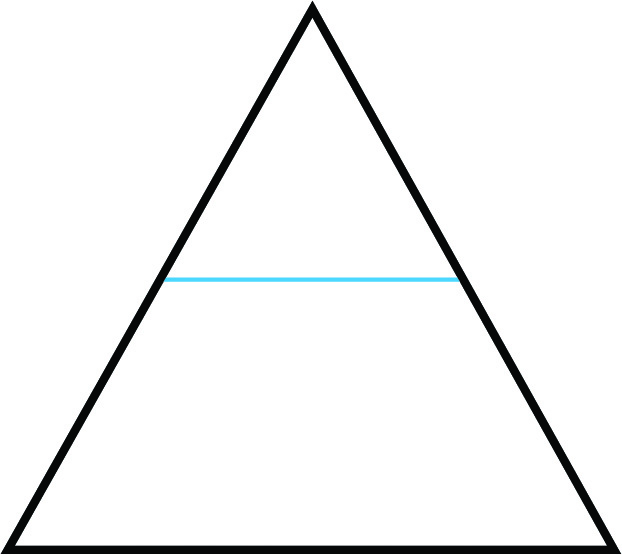
\includegraphics[width=0.2\textwidth]  
			{Tam_giac_6}}
		\hfill
		\subfloat[\textit{\color{toancuabi}Hình} $7$.]{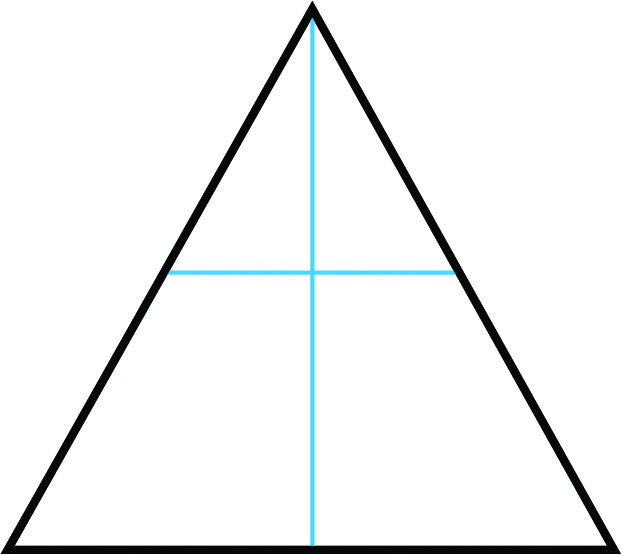
\includegraphics[width=0.2\textwidth]{Tam_giac_7}}
		\hfill
		\subfloat[\textit{\color{toancuabi}Hình} $8$.]{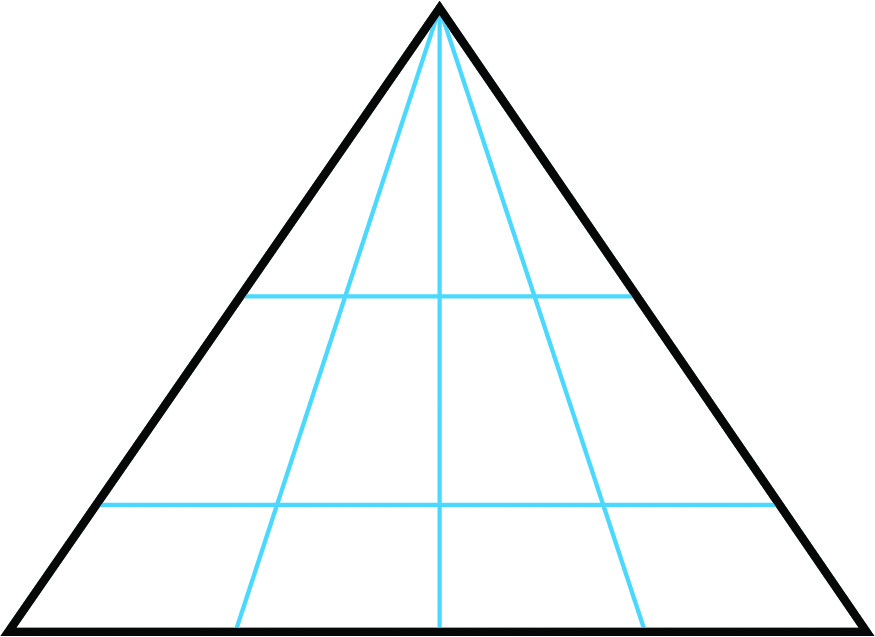
\includegraphics[width=0.2\textwidth]{Tam_giac_8}}
		\hfill
		\vspace*{-10pt}
	\end{figure}    
	\textbf{\color{toancuabi}Lời giải.} Nhận thấy mỗi đường nằm ngang tạo ra một kiểu tam giác và số tam giác cần tìm bằng tổng số tam giác tạo ra theo mỗi đường nằm ngang này. Mặt khác, ta cũng thấy mỗi kiểu tam giác tạo bởi một đường nằm ngang là những tam giác đã đưa ra trong Bài toán $1$.
	\vskip 0.1cm
	Theo Quy tắc $1$, ta có Bảng $2$.
\begin{table}[H]
	\vspace*{-5pt}
\centering
\begin{tabular}{|c|c|c|c|}
	\hline
	\multirow{2}{5em}{\centering{Đường nằm ngang}}&\multicolumn{3}{c|}{Số tam giác}\\
	\cline{2-4}
	&Hình $6$&Hình $7$&Hình $8$\\
	\hline
	Thứ $1$ & $1$ &$1+2$& $1+2+3+4$\\
	\hline
	Thứ $2$ &$1$&$1+2$&$1+2+3+4$\\
	\hline
	Thứ $3$ &  & & $1+2+3+4$\\
	\hline
	Tổng &$2\times 1$ &$2(1+2)=6$&$3(1+2+3+4) = 30$\\
	\hline
\end{tabular}
\captionsetup{labelformat= empty, justification=centering}
\caption{\textit{\color{toancuabi}Bảng $2$.}}
\vspace*{-5pt}
\end{table}
	Từ bảng này, ta cũng có ngay “câu thần chú” thứ hai như sau.
	\vskip 0.1cm
	\textbf{\color{toancuabi}Quy tắc} $\pmb{2.}$ \textit{Số tam giác trong một tam giác mà đỉnh bị chia thành $n$ phần và có $m$ đường nằm ngang là}:
	\begin{align*}
	\color{red}m(1+2+\cdots+n) = \frac{mn(n+1)}{2}.
	\end{align*}
	\begin{figure}[H]
		\centering
		\vspace*{-5pt}
		\captionsetup{labelformat= empty, justification=centering}
		\captionsetup[subfigure]{labelformat=empty}
		\hfill\subfloat[\textit{\color{toancuabi}Hình} $6$.]{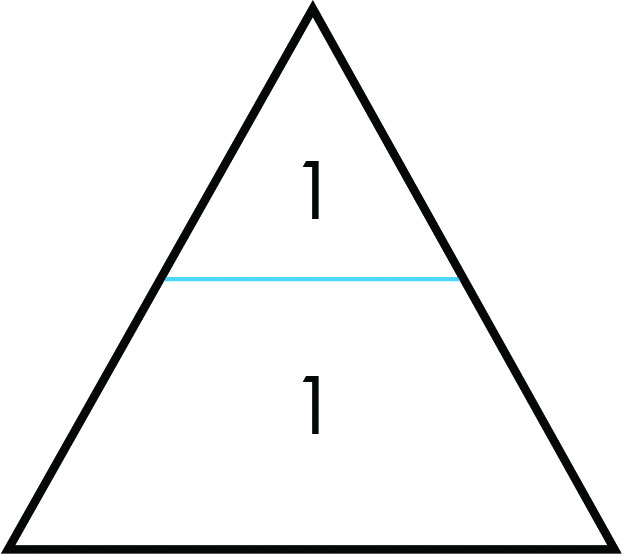
\includegraphics[width=0.15\textwidth]  
			{Tam_giac_6_giai}}\hfill
		\subfloat[\textit{\color{toancuabi}Hình} $7$.]{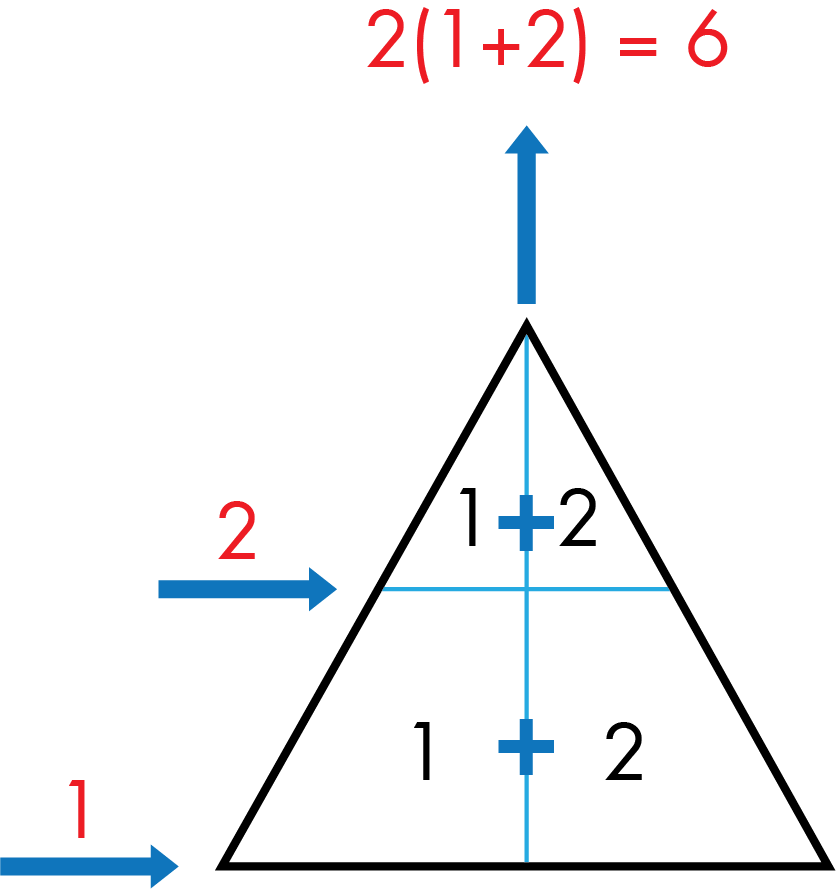
\includegraphics[width=0.2\textwidth]{Tam_giac_7_giai}}\hfill
		\subfloat[\textit{\color{toancuabi}Hình} $8$.]{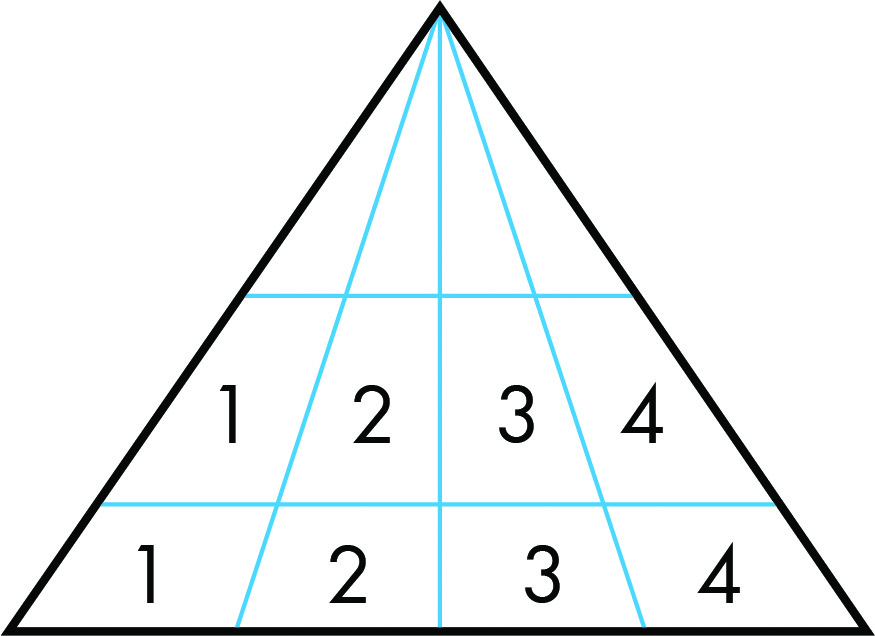
\includegraphics[width=0.2\textwidth]{Tam_giac_8_giai}}\hfill
		\vspace*{-5pt}
	\end{figure} 
	Vận dụng “câu thần chú” thứ hai, các bạn nhỏ hãy giải bài tập sau nhé.
	\vskip 0.1cm
	\textbf{\color{toancuabi}Bài tập} $\pmb{2}$. \textit{Đếm số tam giác trong hai hình dưới đây.}
	\begin{figure}[H]
		\centering
		\vspace*{-5pt}
		\captionsetup{labelformat= empty, justification=centering}
		\captionsetup[subfigure]{labelformat=empty}
		\hfill\subfloat[\textit{\color{toancuabi}Hình} $9$.]{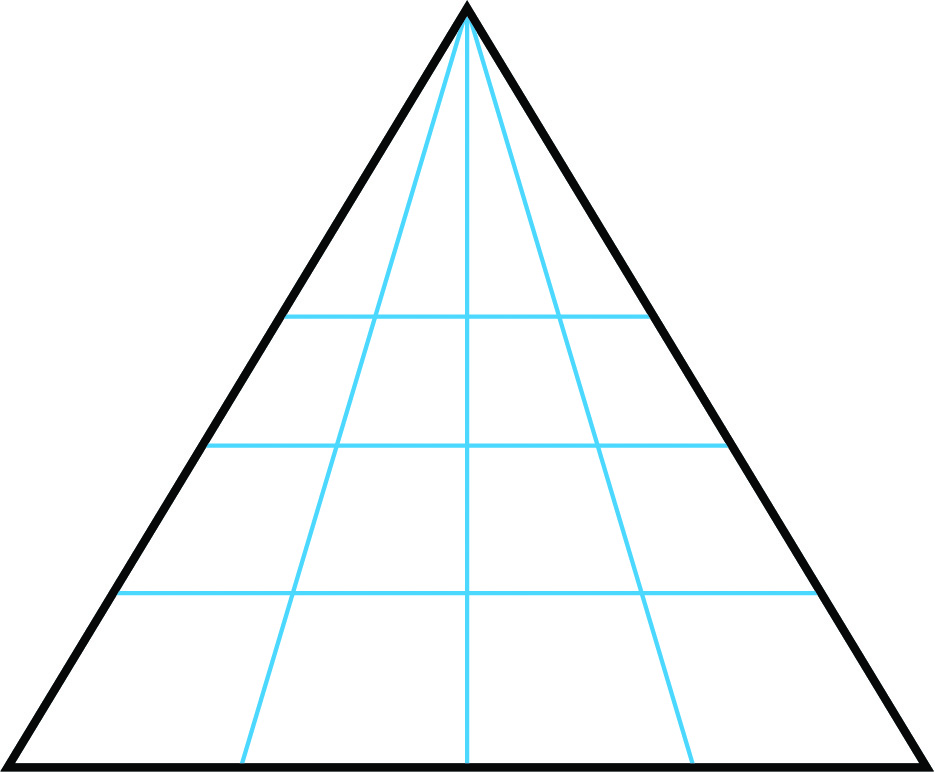
\includegraphics[width=0.15\textwidth]  
			{Tam_giac_9}}
		\hfill
		\subfloat[\textit{\color{toancuabi}Hình} $10$.]{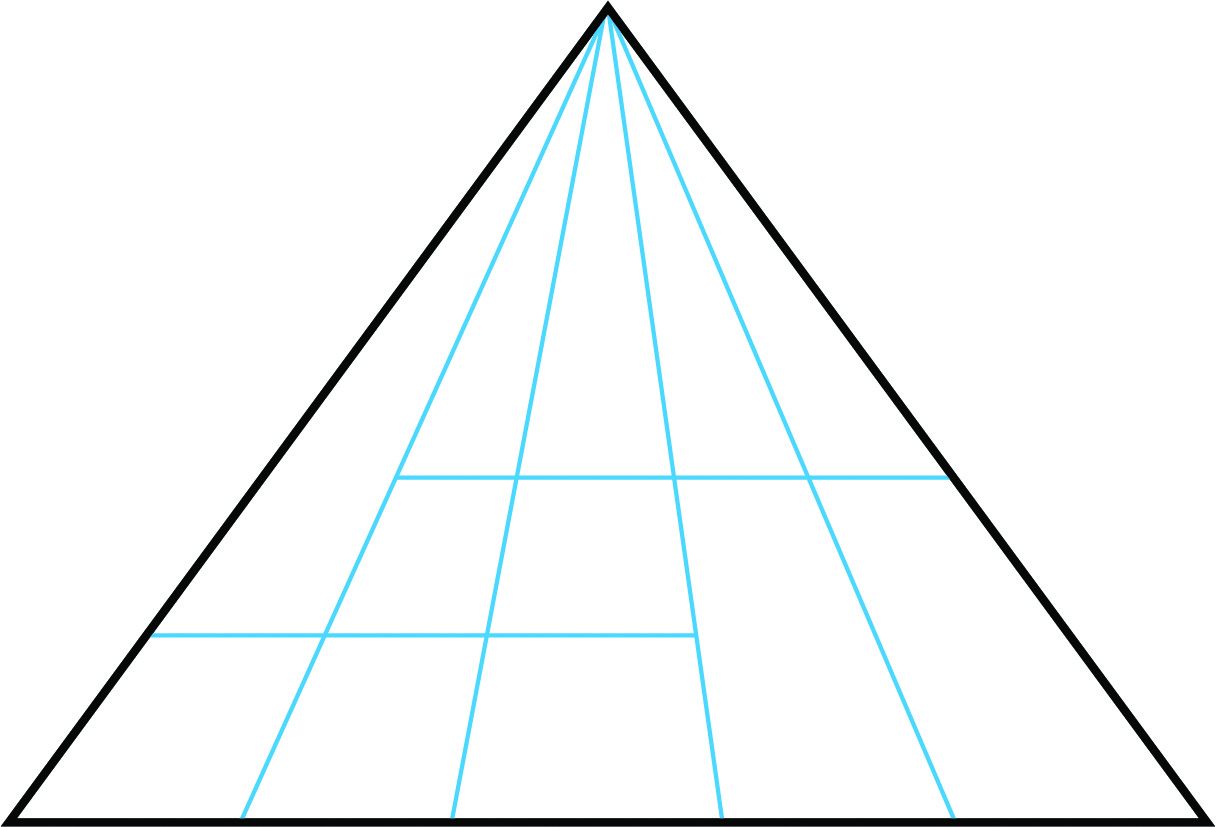
\includegraphics[width=0.2\textwidth]{Tam_giac_10}}\hfill
		\vspace*{-10pt}
	\end{figure} 
	Thế là chúng ta đã hoàn thành được hai nhiệm vụ rồi đấy. Các bạn nhỏ thấy việc tìm “câu thần chú” cũng đơn giản thôi đúng không? Bây giờ, ta cùng thực hiện tiếp nhiệm vụ thứ ba nhé.
	\vskip 0.1cm
	\textbf{\color{toancuabi}Bài toán $\pmb{3.}$ Đếm số tam giác trong hình vuông (hình chữ nhật) tạo thành từ các đường chéo và đường thẳng đi qua giao điểm của các đường chéo.}
	\vskip 0.1cm
	\textbf{\color{toancuabi}Ví dụ} $\pmb{3.}$ \textit{Đếm số tam giác trong các hình dưới đây.}
	\begin{figure}[H]
		\centering
		\vspace*{-5pt}
		\captionsetup{labelformat= empty, justification=centering}
		\captionsetup[subfigure]{labelformat=empty}
		\hfill\subfloat[\textit{\color{toancuabi}Hình $11$}.]{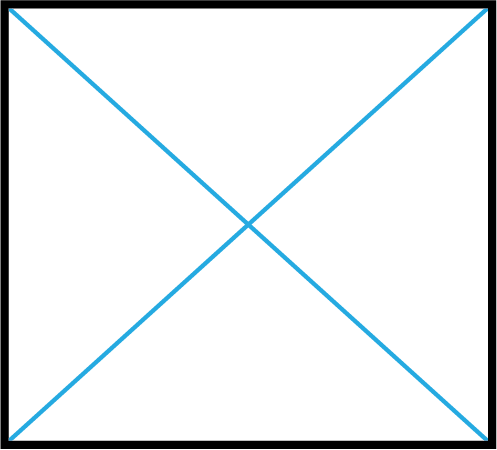
\includegraphics[width=0.15\textwidth]  
			{Tam_giac_11}}
		\hfill
		\subfloat[\textit{\color{toancuabi}Hình $12$}.]{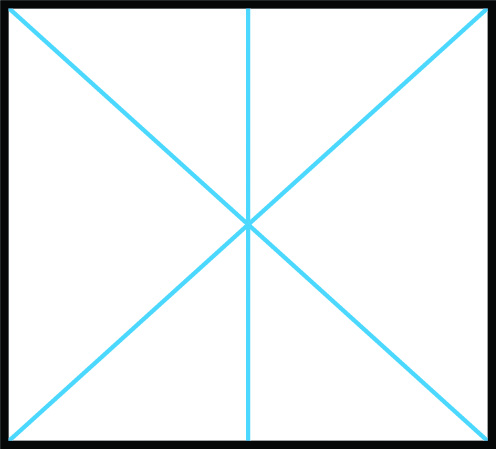
\includegraphics[width=0.15\textwidth]{Tam_giac_12}}
		\hfill
		\subfloat[\textit{\color{toancuabi}Hình} $13$.]{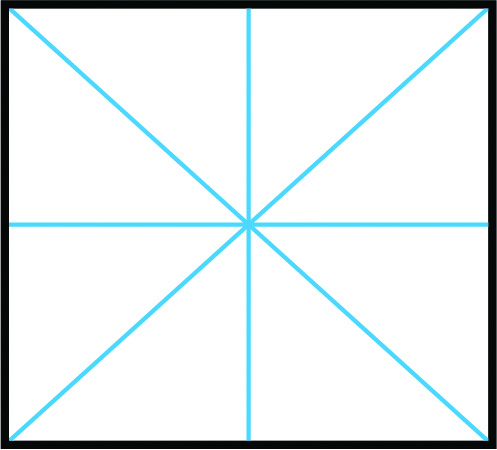
\includegraphics[width=0.15\textwidth]{Tam_giac_13}}
		\hfill
		\subfloat[\textit{\color{toancuabi}Hình} $14$.]{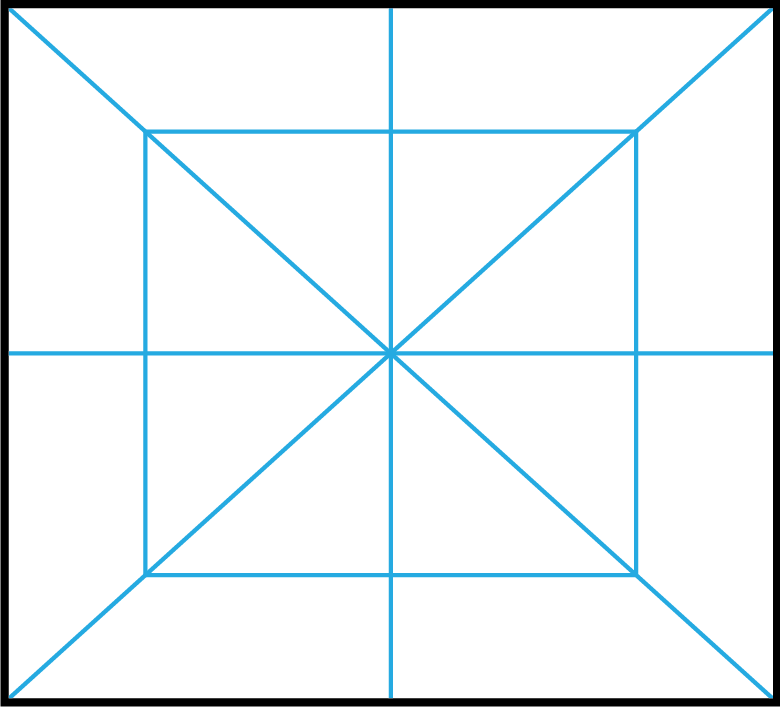
\includegraphics[width=0.15\textwidth]{Tam_giac_14}}
		\hfill
		\vspace*{-10pt}
	\end{figure} 
	\textbf{\color{toancuabi}Lời giải.}
	\vskip 0.1cm
	Bằng cách liệt kê tam giác theo các cách kết hợp hình thông thường, không khó khăn lắm các bạn nhỏ có thể đếm được Hình $11$ có $8$ tam giác, dài hơn một chút thì thấy Hình $12$ có $12$ tam giác. Thế còn Hình $13$ thì sao? Có quy luật gì cho những số tam giác trong những loại hình như thế này không?
	\vskip 0.1cm
	\begin{multicols}{2}
		Nếu đánh số từng tam giác đơn bên trong hình vuông ta thấy.
		\vskip 0.1cm
		Như vậy, ta rút ra một “câu thần chú” đếm tam giác vô cùng đơn giản trong trường hợp này đó là:
		\begin{figure}[H]
			\centering
			\vspace*{-5pt}
			\captionsetup{labelformat= empty, justification=centering}
			\captionsetup[subfigure]{labelformat=empty}
			\hfill\subfloat[\textit{\color{toancuabi}Số tam giác trong Hình~$11$.}]{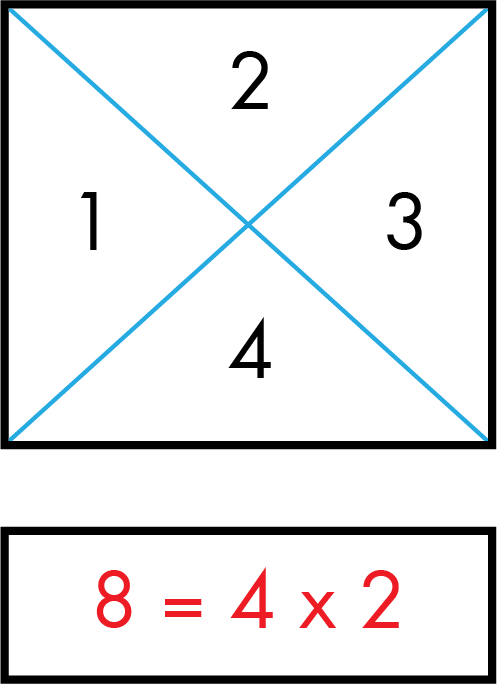
\includegraphics[width=0.15\textwidth]  
				{Tam_giac_11_giai}}
			\hfill
			\subfloat[\textit{\color{toancuabi}Số tam giác trong Hình~$12$.}]{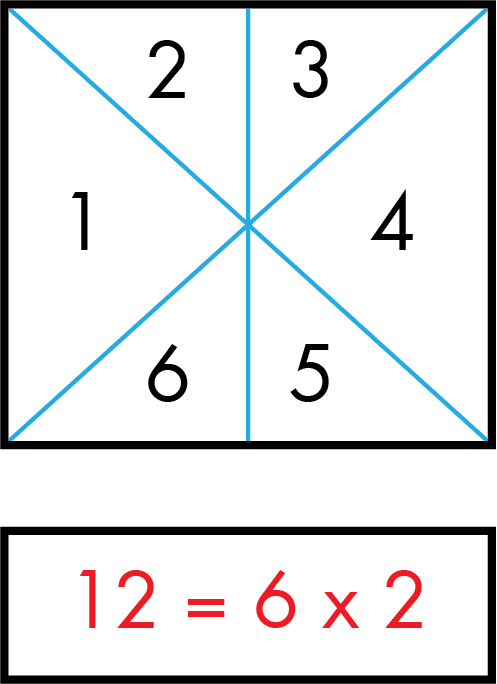
\includegraphics[width=0.15\textwidth]{Tam_giac_12_giai}}\hfill
			\vspace*{-10pt}
		\end{figure} 
	\end{multicols}
	\vskip 0.1cm
	\textbf{\color{toancuabi}Quy tắc} $\pmb{3.}$ \textit{Nếu một hình vuông (hình chữ nhật) bị chia thành $n$ tam giác bởi các đường chéo và một hoặc hai đường thẳng đi qua giao điểm của chúng, trong đó chỉ có một đường thẳng cắt hai cạnh đối diện, thì số tam giác trong hình vuông (hình chữ nhật) là $2n$.}
	\vskip 0.1cm
	\begin{multicols}{2}
		Từ đó, ta có thể đếm một cách nhanh chóng Hình $13$ có $16$ tam giác. Việc đếm số tam giác trong Hình $14$ chính là đếm số tam giác trong hai hình như Hình $13$ và do vậy Hình $14$ có $32$ tam giác như sau.
		\begin{figure}[H]
			\centering
			\vspace*{-15pt}
			\captionsetup{labelformat= empty, justification=centering}
			\captionsetup[subfigure]{labelformat=empty}
			\hfill\subfloat[\textit{\color{toancuabi}Số tam giác trong Hình~$13$.}]{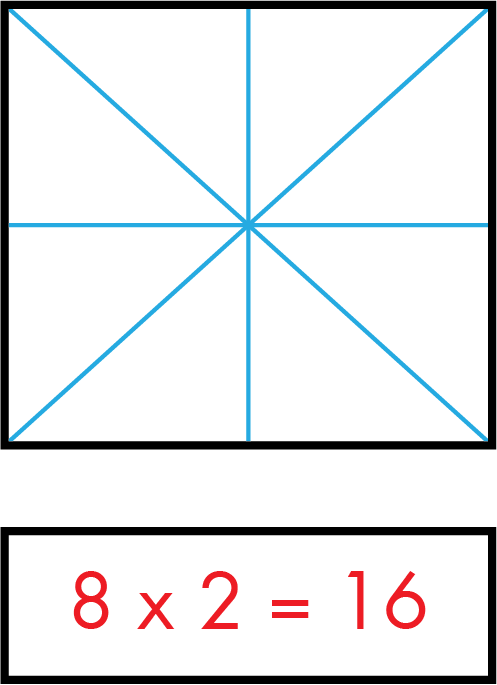
\includegraphics[width=0.2\textwidth]  
				{Tam_giac_13_giai}}
			\hfill
			\subfloat[\textit{\color{toancuabi}Số tam giác trong Hình~$14$.}]{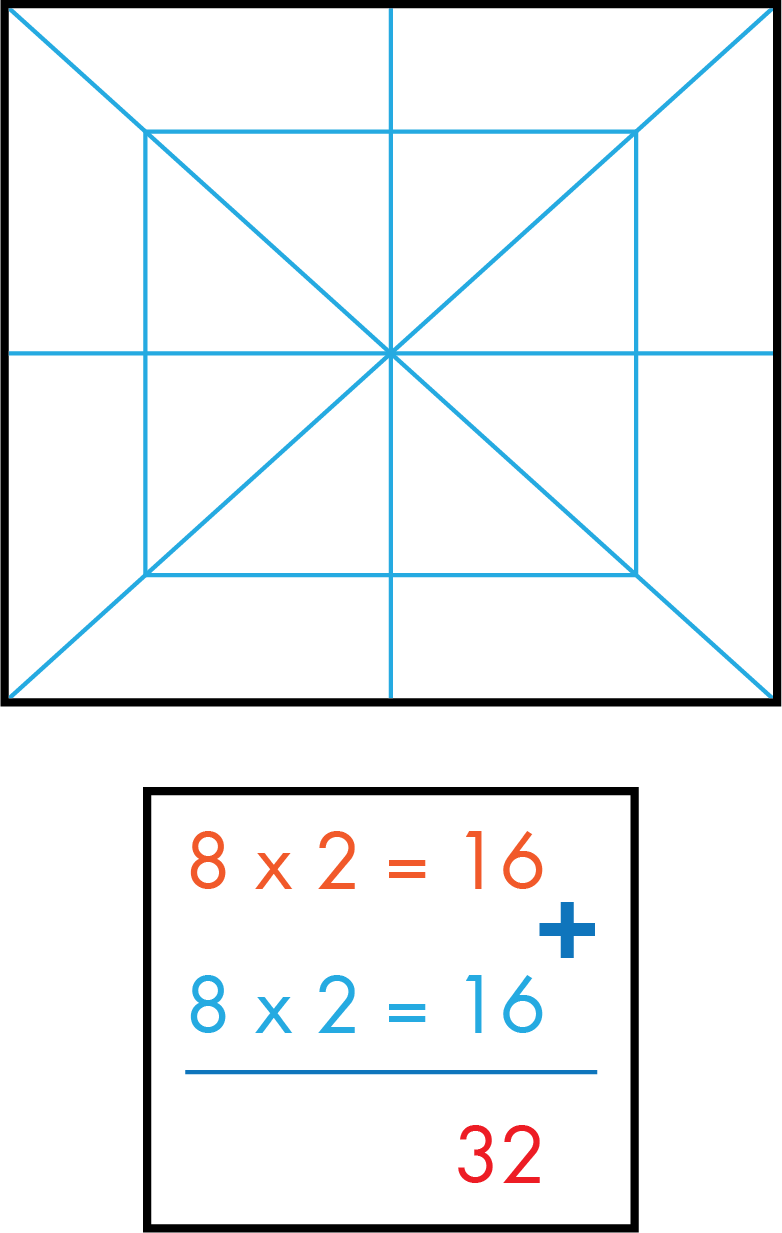
\includegraphics[width=0.2\textwidth]{Tam_giac_14_giai}}\hfill
			\vspace*{-10pt}
		\end{figure} 
	\end{multicols}
	Qua ba nhiệm vụ vừa rồi, các bạn nhỏ đã quen cách tự mình tìm ra “câu thần chú” rồi đúng không. Dưới đây là một bài tập tương tự như Bài toán $3$ ở trên. Các bạn nhỏ hãy đếm hình và đưa ra “câu thần chú” nhé.
	\vskip 0.1cm
	\textbf{\color{toancuabi}Bài tập} $\pmb{3}$. \textit{Hãy đếm số tam giác trong các hình sau và rút ra quy luật.}
	\begin{figure}[H]
		\centering
		\vspace*{-5pt}
		\captionsetup{labelformat= empty, justification=centering}
		\captionsetup[subfigure]{labelformat=empty}
		\hfill\subfloat[\textit{\color{toancuabi}Hình} $15$.]{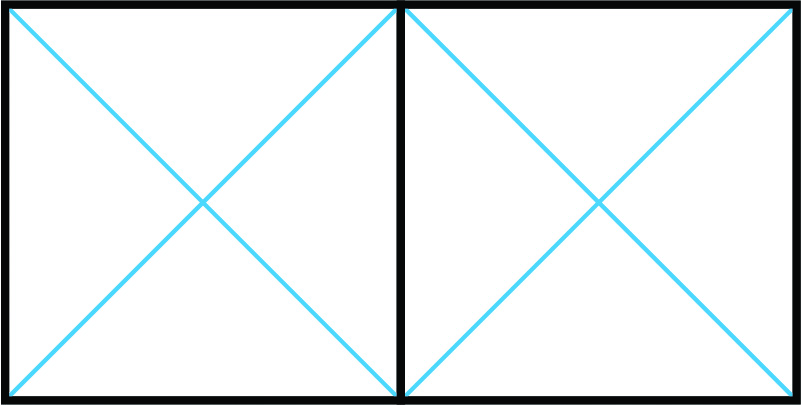
\includegraphics[width=0.25\textwidth]  
			{Tam_giac_15}}\hfill
		\subfloat[\textit{\color{toancuabi}Hình} $16$.]{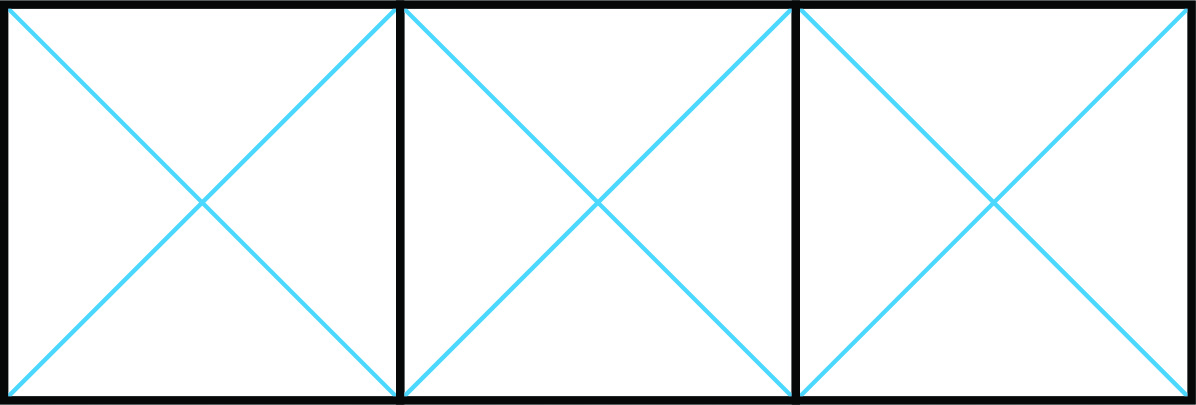
\includegraphics[width=0.37\textwidth]{Tam_giac_16}}\hfill
		\vspace*{-5pt}
	\end{figure} 
